\documentclass[conference]{llncs}

\usepackage{url}
\usepackage{amsmath}
\usepackage{graphicx}
\usepackage{subfigure}
\usepackage{threeparttable}
\usepackage{pdflscape}
\usepackage{array}

\begin{document}

\title{Dismal Code: Studying the Evolution of Security Bugs}

\author{Dimitris Mitropoulos \and Vassilios Karakoidas \and Panos Louridas \and Georgios Gousios \and Diomidis Spinellis }
\institute{ Department of Management Science and Technology\\
			Athens University of Economics and Business\\
      		\email{\{dimitro, bkarak, louridas, dds\}@aueb.gr}\\
			Software Engineering Research Group\\
			Delft University of Technology\\
			\email{G.Gousios@tudelft.nl}}

\maketitle

\begin{abstract}
%\boldmath
Security bugs are critical programming errors that can lead to serious
vulnerabilities in software. Such bugs may allow an attacker to take over
an application, steal data or prevent the application from working at all.
In this paper, we present how we used the Maven repository to study the
characteristics of security bugs individually and in relation to other software
bugs. In particular, we analyzed every project version of the repository by using a
popular static analysis tool. Then by taking advantage of the various features of
the repository (multiple versions for every project, dependencies and others) we studied
the evolution of security bugs through time, their persistence and their relationship with a) the
size of the corresponding version and b) other bug categories. Also, based on the
dependencies of artifacts we constructed the graph of the repository and
examined the most popular nodes based on their PageRank. 
\end{abstract}

\begin{keywords}
Security Bugs, Static Analysis, Software Evolution, Software
Security, Maven, FindBugs.
\end{keywords}

\section{Introduction}

A security bug is a programming error that introduces a potentially
exploitable weakness into a computer system~\cite{SSL12}\cite{TJBD11}\cite{M06}. This weakness could lead to a
security breach with unfortunate consequences in different layers, like databases,
native code, applications, libraries and others. Despite the significant
effort to detect and eliminate such bugs~\cite{SZ12}, little attention has been paid to
study them in relation to software evolution~\cite{L96}\cite{LRWPT97}\cite{IB06}\cite{RGMA06}.
In this paper we present how we used a large software ecosystem to analyse
how evolving software packages are related to the different types of security
vulnerabilities.

One of the most common approaches to identify security bugs is
{\it static analysis}~\cite{CW07}. This kind of analysis involves the
inspection of the program's source or object code without executing
it. For our research we used {\it FindBugs},\footnote{\url{http://findbugs.sourceforge.net/}}
a static analysis tool that examines bytecode to detect software bugs and has already been used in
research~\cite{AP10}\cite{HP07}\cite{HP04}\cite{HW08}\cite{SHP06}.
Specifically, we ran FindBugs on all the project
versions of all the projects that exist in the
{\it Maven Central Repository}\footnote{\url{http://search.maven.org/}}
(approximately 265GB of data - see Section~\ref{sec:data}).
Then we observed the changes that involved the security bugs and their characteristics.
This research builds upon our earlier work on the topic~\cite{MGS12}.

We chose to focus our study on the security bugs rather than other
software bugs. This is because compared to other bug categories,
the category of security bugs has two distinct features: it is critical~\cite{SZ12}
and it costs~\cite{BCL08}\cite{R06}. Specifically, a software bug can
lead to a malfunction of a software artifact that runs under specific
requirements but a security bug can allow a malicious user to alter the execution
of the entire application for his or her own gain. In this case, such bugs could span a wide
range of security and privacy issues, like viewing sensitive information, the destruction or
modification of sensitive data, denial of service and others.
Moreover, security bug disclosures lead to a negative and significant change
in market value for a software vendor~\cite{TW07}.
Hence, one of the basic pursuits in every new software release should
be the mitigation of such bugs.

The motivation behind our work was to validate if programmers tend to care for
such high-risk bugs when they release a new version of their software. In
addition, we wanted to investigate other critical features associated with such
vulnerabilities like the persistence of a bug. In essence, to check if critical bugs stay
unresolved for a long time. Also, we wanted to elaborate more on the relation of security
bugs not only with performance bugs (as Zaman et al.~\cite{ZAH11} have already
did) but also with other bug categories. In the same manner, we tried to check
the relation between a version's size and its' security bugs knowing the
that research has been contradictory on the the
issue~\cite{BP84}\cite{SYTP85}\cite{NBZ06}\cite{GKMS00}.
Finally, we examined the Maven ecosystem as a whole from a security
perspective. Its structure, gave us the opportunity to see if a project version that is a dependency to
a large number of others contains a low rate of security bugs~\cite{MW10}.
%In this case we can strengthen the relationship between Linus' Law and
%software security as Meneely et al. have already indicated~\cite{MW10}.

The main contributions of this research are:
\begin{itemize}
	\item The analysis of how security bugs evolve over time. To achieve
this, we inspect every project per version. We expect that security
bugs should decrease as a project evolves since they are critical and developers
should eliminate them.
	\item Security bug persistence between versions. We show evidence that
security bugs are not eliminated between versions.
	\item We show evidence of the relation between security bugs and a project
version's size.  Here, size is defined in terms of bytecode.
	\item The correlation of security bugs with other bug categories. We
show evidence on how such bugs are correlated with bugs that have to do with
performance, coding practices and others.
%	\item The relation of software dependencies and security bugs. Our
%hypothesis is that an artifact that is a dependency of many other artifacts
%should have a low rate of security bugs. 
\end{itemize}

% In the rest of this paper we
% describe the processing of our data and our experiment (Section \ref{sec:meth}),
% present and discuss the results we obtained (Section \ref{sec:res}),
% outline related work (Section \ref{sec:rel}),
% and end up with a conclusion and directions for future work (Section \ref{sec:con}).

\section{Methodology}
\label{sec:meth}

Our experiment involved the collection of the metric results of the FindBugs
tool. Before and during the experiment, we performed a number of functional
fits on the data coming from the Maven repository, for reasons that we will describe below.

\subsection{Experiment}
\label{sec:exp}

Our experiment involved four entities (see Table~\ref{tbl:exp}):
a number of {\it workers}, a {\it task queue}
mechanism,\footnote{\url{http://www.rabbitmq.com/}}
a {\it data repository},\footnote{\url{http://www.mongodb.org/}}
and the {\it code repository}, which in our case it was
the public Maven repository.

\begin{table}
\centering
\begin{threeparttable}
\caption{Experiment Entities}
\label{tbl:exp}
\begin{tabular}{l r r}
\hline
Entity & Software Package & Version\\
\hline
Worker & Custom Python Script & 2.7\\
Task Queue & RabbitMQ & 3.0.1 \\
Data Repository & MongoDB & 2.2 \\
Code Repository & Maven Central Repository & January 2012 \\
\hline
\end{tabular}
\end{threeparttable}
\end{table}

First, we scanned the Maven repository for appropriate {\sc jar}s and created a
list that included them. We discuss the {\sc jar} selection process in the next 
section. With the {\sc jar} list at hand, we created a series of processing tasks
and added them to the task queue. Then we executed twenty five (Unix-based)
workers that checked out tasks from the queue, processed the data and stored the
results to the data repository.

\begin{figure}[t]
  \begin{center}
    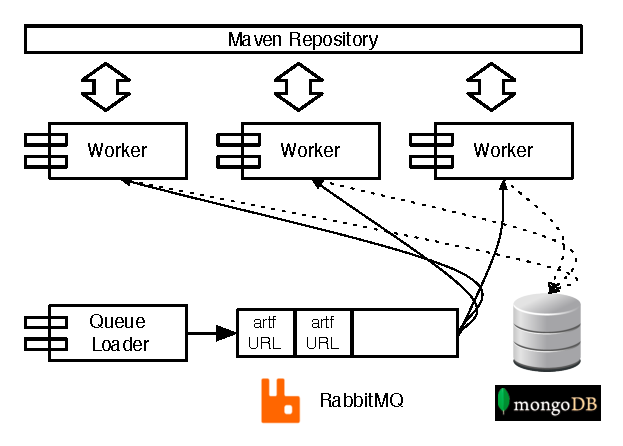
\includegraphics[scale=0.7]{figures/arch.pdf}
  \end{center}
  \caption{The Data Processing Architecture}
  \label{fig:arch}
\end{figure}

A typical processing cycle of a worker included the following steps: after
the worker spawned, it requested a task from the queue. This task contained
the {\sc jar} name, which was typically a project version that was downloaded locally.
First, specific {\sc jar} metadata were calculated and stored. Such metadata included
its size, its dependencies, and a number that represented the chronological order of the
release. This order was derived from an {\sc xml} file that
accompanies every project in the Maven repository called {\it
maven-metadata.xml}. Then, FindBugs was invoked by the worker and its results were
also stored in the data repository. When the task was completed the queue
was notified and the next task was requested. A schematic representation
of the data processing architecture can be seen in Figure~\ref{fig:arch}.

This process was executed for all the available {\sc jar}s in the task queue.
The experiment was executed five times in order to iron out various bugs in
our scripts and validate the results. 

\subsection{Data Provenance}
\label{sec:data}

Maven is a build automation tool used primarily for Java projects and it is
hosted by the Apache Software Foundation.\footnote{\url{http://www.apache.org/}}
To describe the software project being built, its dependencies
on other external modules, the build order, and required plug-ins Maven uses
{\sc xml}. To build a software component, it dynamically downloads Java libraries
and Maven plug-ins from the Maven central repository,
and stores them in a local cache. The repository can be updated with
new projects and also with new versions of existing projects.

Initially, we obtained a snapshot (January 2012) of the Maven repository and
handled it locally to retrieve a list of all the names of the project versions
that existed in it. A project version can be uniquely identified by the triplet:
{\it group id}, {\it artifact id} and {\it version}.
Since FindBugs analyses applications written in the Java
programming language, and the Maven repository
hosts projects from languages other than Java such as Scala, Groovy,
Clojure etc. we filtered out such projects by performing a series of checks in
the repository data and metadata.

\begin{table}
\centering
\caption{Descriptive Statistics Measurements for the Maven Repository}
\label{tbl:repository}
\begin{tabular}{l r}
\hline
Measurement & Value\\
 \hline
Projects & 17,505\\
Versions (total) & 115,214\\
Min & 1\\
Max & 338\\
Mean & 6.58\\
Median & 3\\
Range & 337\\
1$^{st}$ Quartile & 1\\
3$^{rd}$ Quartile & 8\\
\hline
\end{tabular}
\end{table}

In addition, we implemented a series of audits in the worker scripts that
checked if the {\sc jar}s are valid in terms of implementation. For instance,
for every {\sc jar} the worker checked if there were any {\it .class} files
before invoking FindBugs. After the project filtering, we narrowed down
our data set to 17,055 projects with 115,214 versions.
Table~\ref{tbl:repository} summarises the data set information and
provides the basic descriptive statistic measurements. The distribution of version
count among the selected projects is presented in Figure \ref{fig:version-count}.

\begin{figure*}
	\centering
	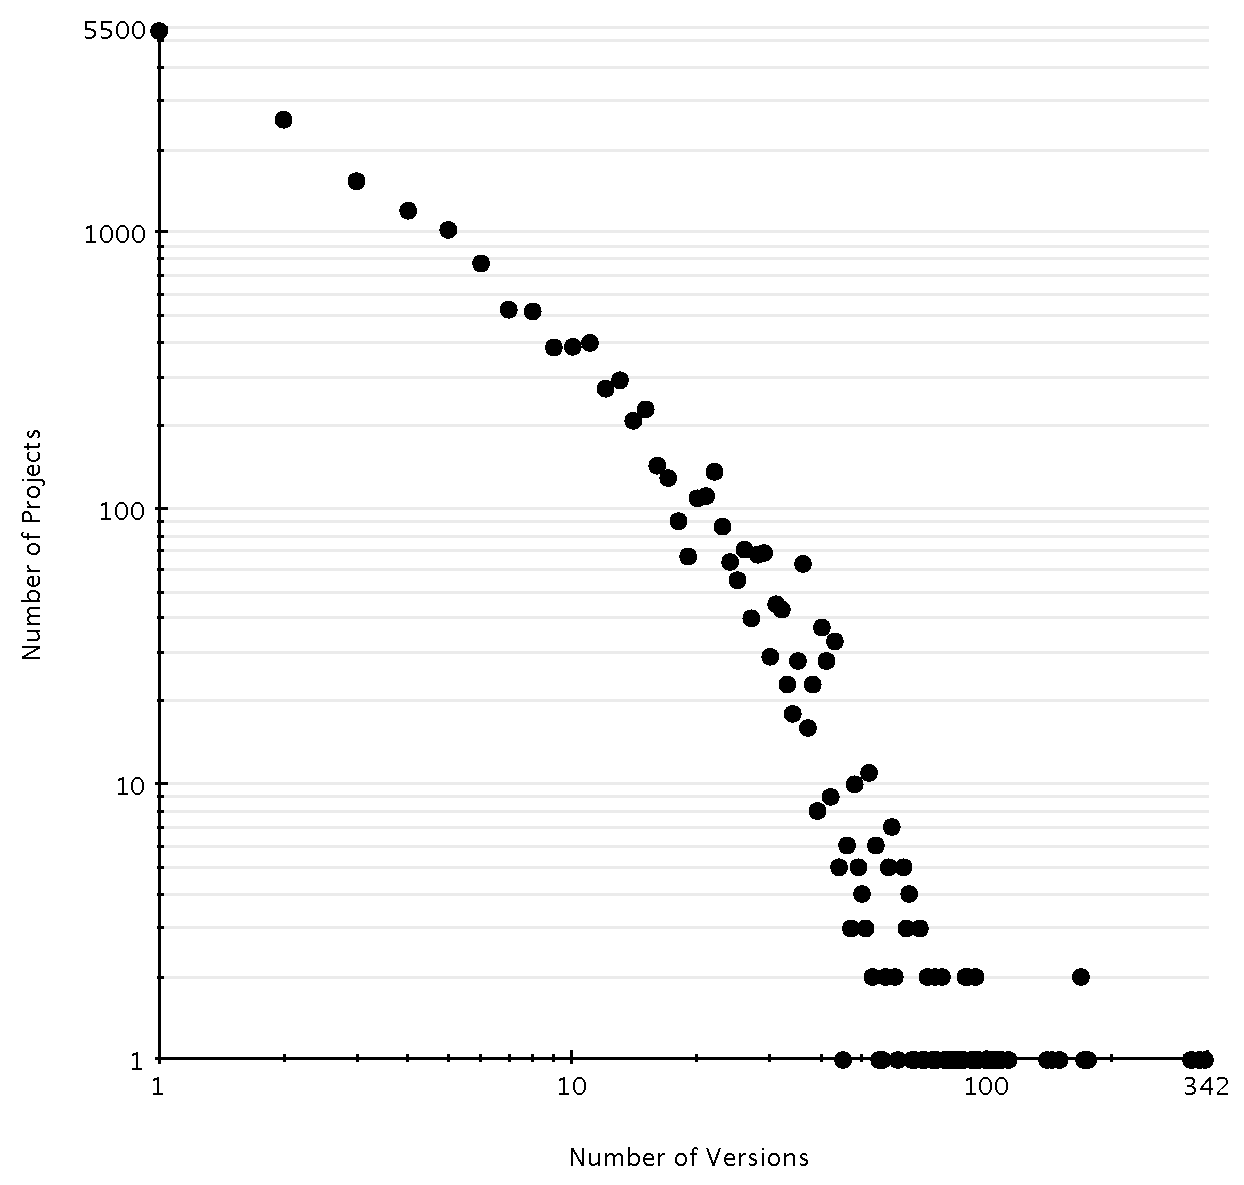
\includegraphics[scale=0.6]{version_count.pdf}
	\caption{Distribution of
Version Count Among Project Population}
	\label{fig:version-count}
\end{figure*}

The statistical measurements presented in Table~\ref{tbl:repository}
indicate that we have 17,505 projects and the data set's median
is 3, which means that almost 50\% (8,753 projects) of the project
population has 1 to 3 versions.
Note that the Maven repository has many projects with a
few number of versions. For instance, there are numerous projects with a
number of versions that is less than ten.
There are a few projects containing ten
versions and only a few with hundreds of versions. The maximum number of
versions for a project is 338. The 3$^{rd}$ quartile measurement
also indicated that 75\% (13,129) of the projects have a maximum of 8 versions.

\section{Results and Analysis}
\label{sec:res}

\begin{table}
\centering
\caption{Bug Categorisation According to FindBugs}
\label{tbl:bug-cat}
\begin{tabular}{l p{15em}}
\hline
Category & Description\\
\hline
Bad Practice & Violations of recommended and essential
coding practice. \\
Correctness & Involves coding mistakes resulting in code
that was probably not what the developer intended. \\
Experimental & Includes unsatisfied obligations. For instance,
forgetting to close a file. \\
Internationalization (i18n) & Indicates the use of non-localized methods. \\
Multi-Threaded ({\sc mt}) Correctness & Thread synchronization issues. \\
Performance & Involves inefficient memory usage allocation, usage 
of non-static classes. \\
Style & Code that is confusing, or
written in a way that leads to errors.\\
Malicious Code & Involves variables or fields exposed to classes that should
not be using them. \\
Security & Involves input validation issues, unauthorized database connections
and others. \\
\hline
\end{tabular}
\end{table}

Our findings can be analysed at two levels. First, we discuss some
primary observations concerning the security bugs of the Maven repository as a whole.
Then, we provide a comprehensive analysis of the results and highlight our key findings.

\subsection{Overview and Initial Results}
\label{sec:overview}

FindBugs separates software bugs into nine categories (see
Table~\ref{tbl:bug-cat}). Two of them involve security issues: {\it Security} and {\it
Malicious Code}. From the total number of versions, 4,353 of them contained
at least one bug coming from the first category
and 45,559 coming from the second.

\begin{table*}
\centering
\caption{Number of Versions that Contain at Least One Severe Security Bug}
\label{tbl:sev}
\leavevmode
	\begin{tabular}{l r}
	\hline
	Bug Description & Number of Versions\\
 	\hline
	{\sc hrs}: {\sc http} cookie formed from untrusted input & 149\\
	{\sc hrs}: {\sc http} response splitting vulnerability & 1,564\\
	{\sc pt}: absolute path traversal in servlet  & 92\\
	{\sc pt}: relative path traversal in servlet & 50\\
	{\sc sql}: non-constant string passed to execute method on an {\sc sql} & 1,817\\
	{\sc sql}: a prepared statement is generated from a non-constant String & 1,438\\
	{\sc xss}: {\sc jsp} reflected cross site scripting vulnerability & 17\\
	{\sc xss}: Servlet reflected cross site scripting vulnerability in error page & 88\\
	{\sc xss}: Servlet reflected cross site scripting vulnerability & 140\\
	\hline
	\end{tabular}
\end{table*}

Figure~\ref{fig:bug-per} shows how software bugs are distributed among the
repository. Together with the {\it Bad Practice} bugs and the {\it Style} bugs,
security bugs (the sum of the {\it Security} and {\it Malicious Code}
categories) are the most popular in the repository ($\geq 22\%$ each).
% An interesting observation is that 4,908 projects did not
% have any bugs at all. These cases involved small artifacts with a minimum number of classes.
% This goes along with the relationship between the size of an artifact and it's
% bugs that is presented in the upcoming section.

% dimitro@dds: maybe you want to add something here?
Another observation involves bugs that we could call {\it
severe} and they are a subset of the {\it Security} category.
Such bugs are related to vulnerabilities that appear due to the lack of user-input
validation and can lead to damaging attacks like {\sc sql} injection~\cite{RL12} and
Cross-Site Scripting~\cite{WS08}. Note that to exploit such vulnerabilities, a malicious user does
not have to know anything about the applications internals. For all the other
bugs, another program should be written either to incorporate references to
mutable objects, access non-final fields and others. Table~\ref{tbl:sev} presents the number
of {\sc jar}s where at least one of these bugs exists. In the following section
we provide results separately for this subcategory which we call {\it Security High}.
The remaining bugs of the {\it Security} category
are grouped together with the bugs of the {\it Malicious Code} category
in another subcategory that we call {\it Security Low}.

\begin{figure*}
	\centering
	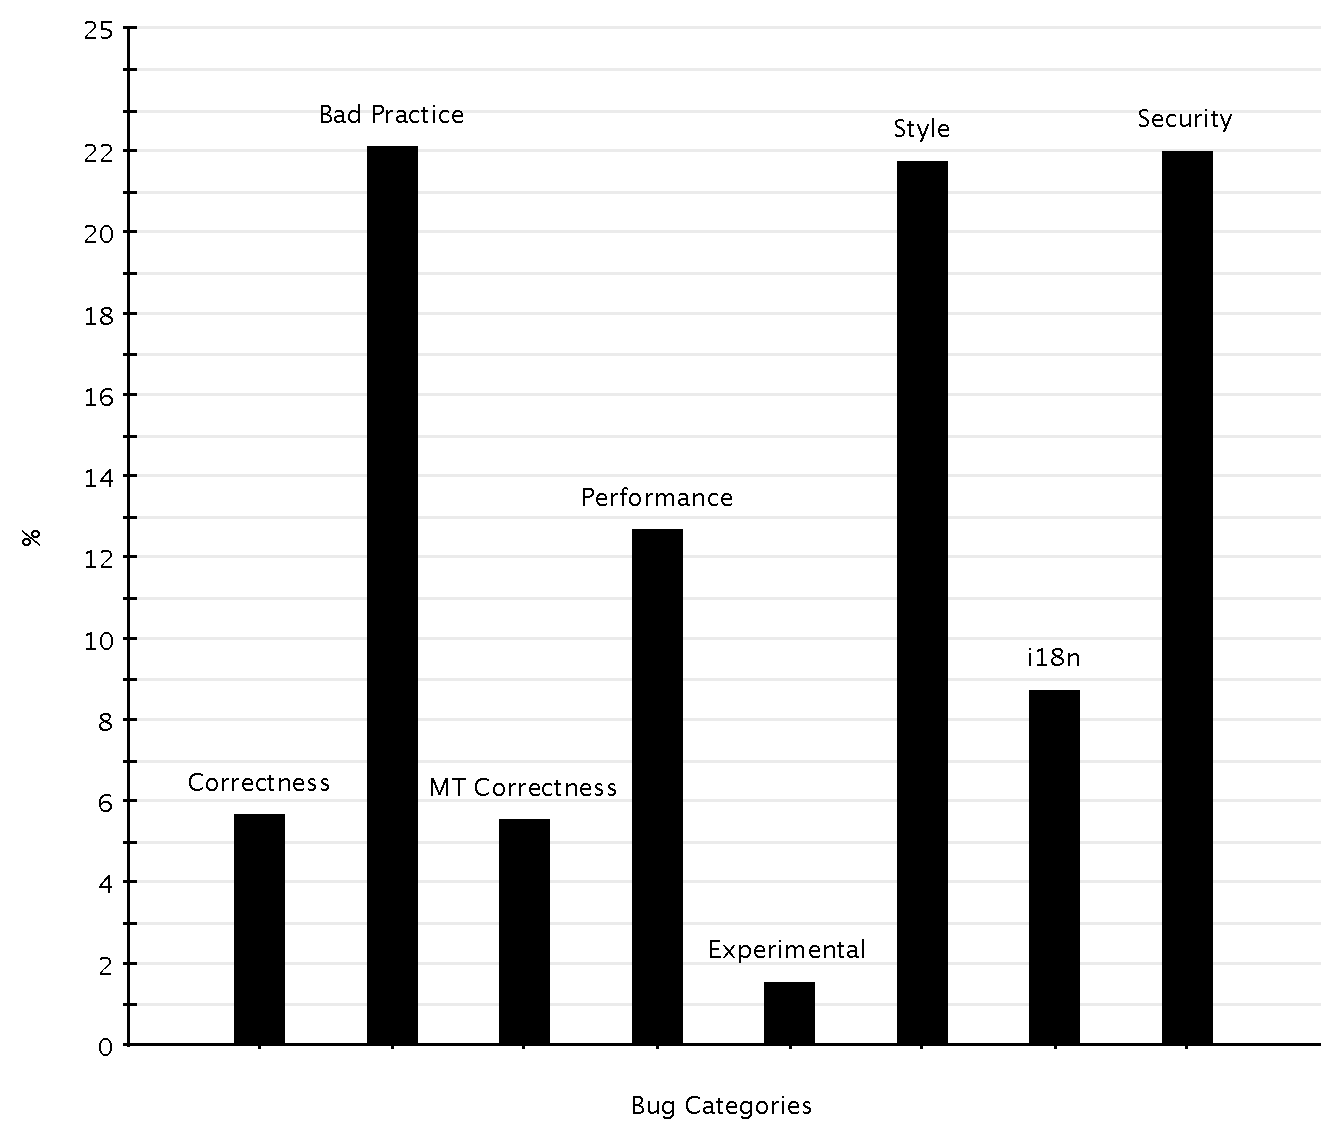
\includegraphics[scale=0.6]{bug_percent}
	\caption{Bug Percentage in Maven Repository}
	\label{fig:bug-per} 
\end{figure*}

As we mentioned earlier, during the experiment we managed to retrieve the
dependencies of every version. Based on this information we created a graph
that represented the snapshot of the Maven repository. The
nodes of the graph represented the versions and the vertices their dependencies.
We have to mention here that the graph was not representative. For instance, if
a dependency was pointing only to a project (and not to a specific version), we chose to
select the latest version found on the repository. Also, this graph is not
complete. This is because there were missing versions.
% Practically, the corresponding {\it pom}, or {\it war} files existed on the
% repository, but the {\sc jar} file did not.
From the 565,680 vertices, 191,433
belonged to the first case while 164,234 belonged to the second.
The graph contained 80,354 nodes. Obviously, the number does not correspond to
the number of the total versions (see Section~\ref{sec:data}). This is because
some versions did not contain any information about their dependencies so they
are not represented in the graph. After creating the graph, we ran the PageRank
algorithm~\cite{BP98} on it and retrieved all PageRanks for every node. Then we
examined the security bugs of the fifty most popular nodes based on their PageRank.
Thirty three of them contained bugs coming from the {\it Security Low} subcategory,
while two of them contained severe bugs. Twenty five of them were latest
versions at the time.
% what can we say about this?

\subsection{Analysis}
\label{sec:analysis}

\subsubsection{How Security Bugs Evolve Over Time}

The relation between bugs and time can be traced from the number of
bugs per category in each project version. We can then calculate the
correlations between the defects count and the ordinal version number
across all projects to see if bigger versions relate to higher or
lower defect counts. The results are shown in
Table~\ref{tbl:bugsperversion}. Although the tendency is for
defect counts to increase, this tendency is extremely slight.
\begin{table}
    \centering
    \caption{Correlations between Version and Defects Count}
    \label{tbl:bugsperversion}
    
\begin{tabular}{lcc}
\hline \\
Category & Spearman Correlation & $p$-value \\ \hline 
Security High & 0.08 & $\ll 0.05$\\
Security Low & 0.02 & $\ll 0.05$\\
Style & 0.03 & $\ll 0.05$\\
Correctness & 0.04 & $\ll 0.05$\\
Bad Practice & 0.03 & $\ll 0.05$\\
MT Correctness & 0.09 & $\ll 0.05$\\
i18n & 0.06 & $\ll 0.05$\\
Performance & {\it (0.01) } & 0.07\\
Experimental & 0.09 & $\ll 0.05$\\
\hline \\
\end{tabular}

\end{table}

Although there seems to be zero tendency taken over all versions of
all projects together, the situation might be different in individual
projects. We therefore performed Spearman correlations between bug
counts and version ordinals in all projects we examined. These paint a
different picture from the above table, shown in
Figure~\ref{fig:bugsversionscorr}. The spike in point zero is
explained by the large number of projects for which no correlation
could be established---note that the scale is logarithmic. Still, we
can see that there were projects where a correlation could be
established, either positive or negative. The {\it Security High}
category is particularly bimodal, but this is explained by the small
number of correlations that could be established, nine in total. Taken
together with Table~\ref{tbl:bugsperversion},
Figure~\ref{fig:bugsversionscorr} suggests that we cannot say that across
projects defect counts increase or decrease significantly across time.
In individual projects, however, defect counts can have a strong
upwards or downwards tendency. There may be no such thing as a
``project'' in general, only particular projects with their own
idiosyncrasies, quality features, and coding practices.

\begin{figure*}
  \centering
  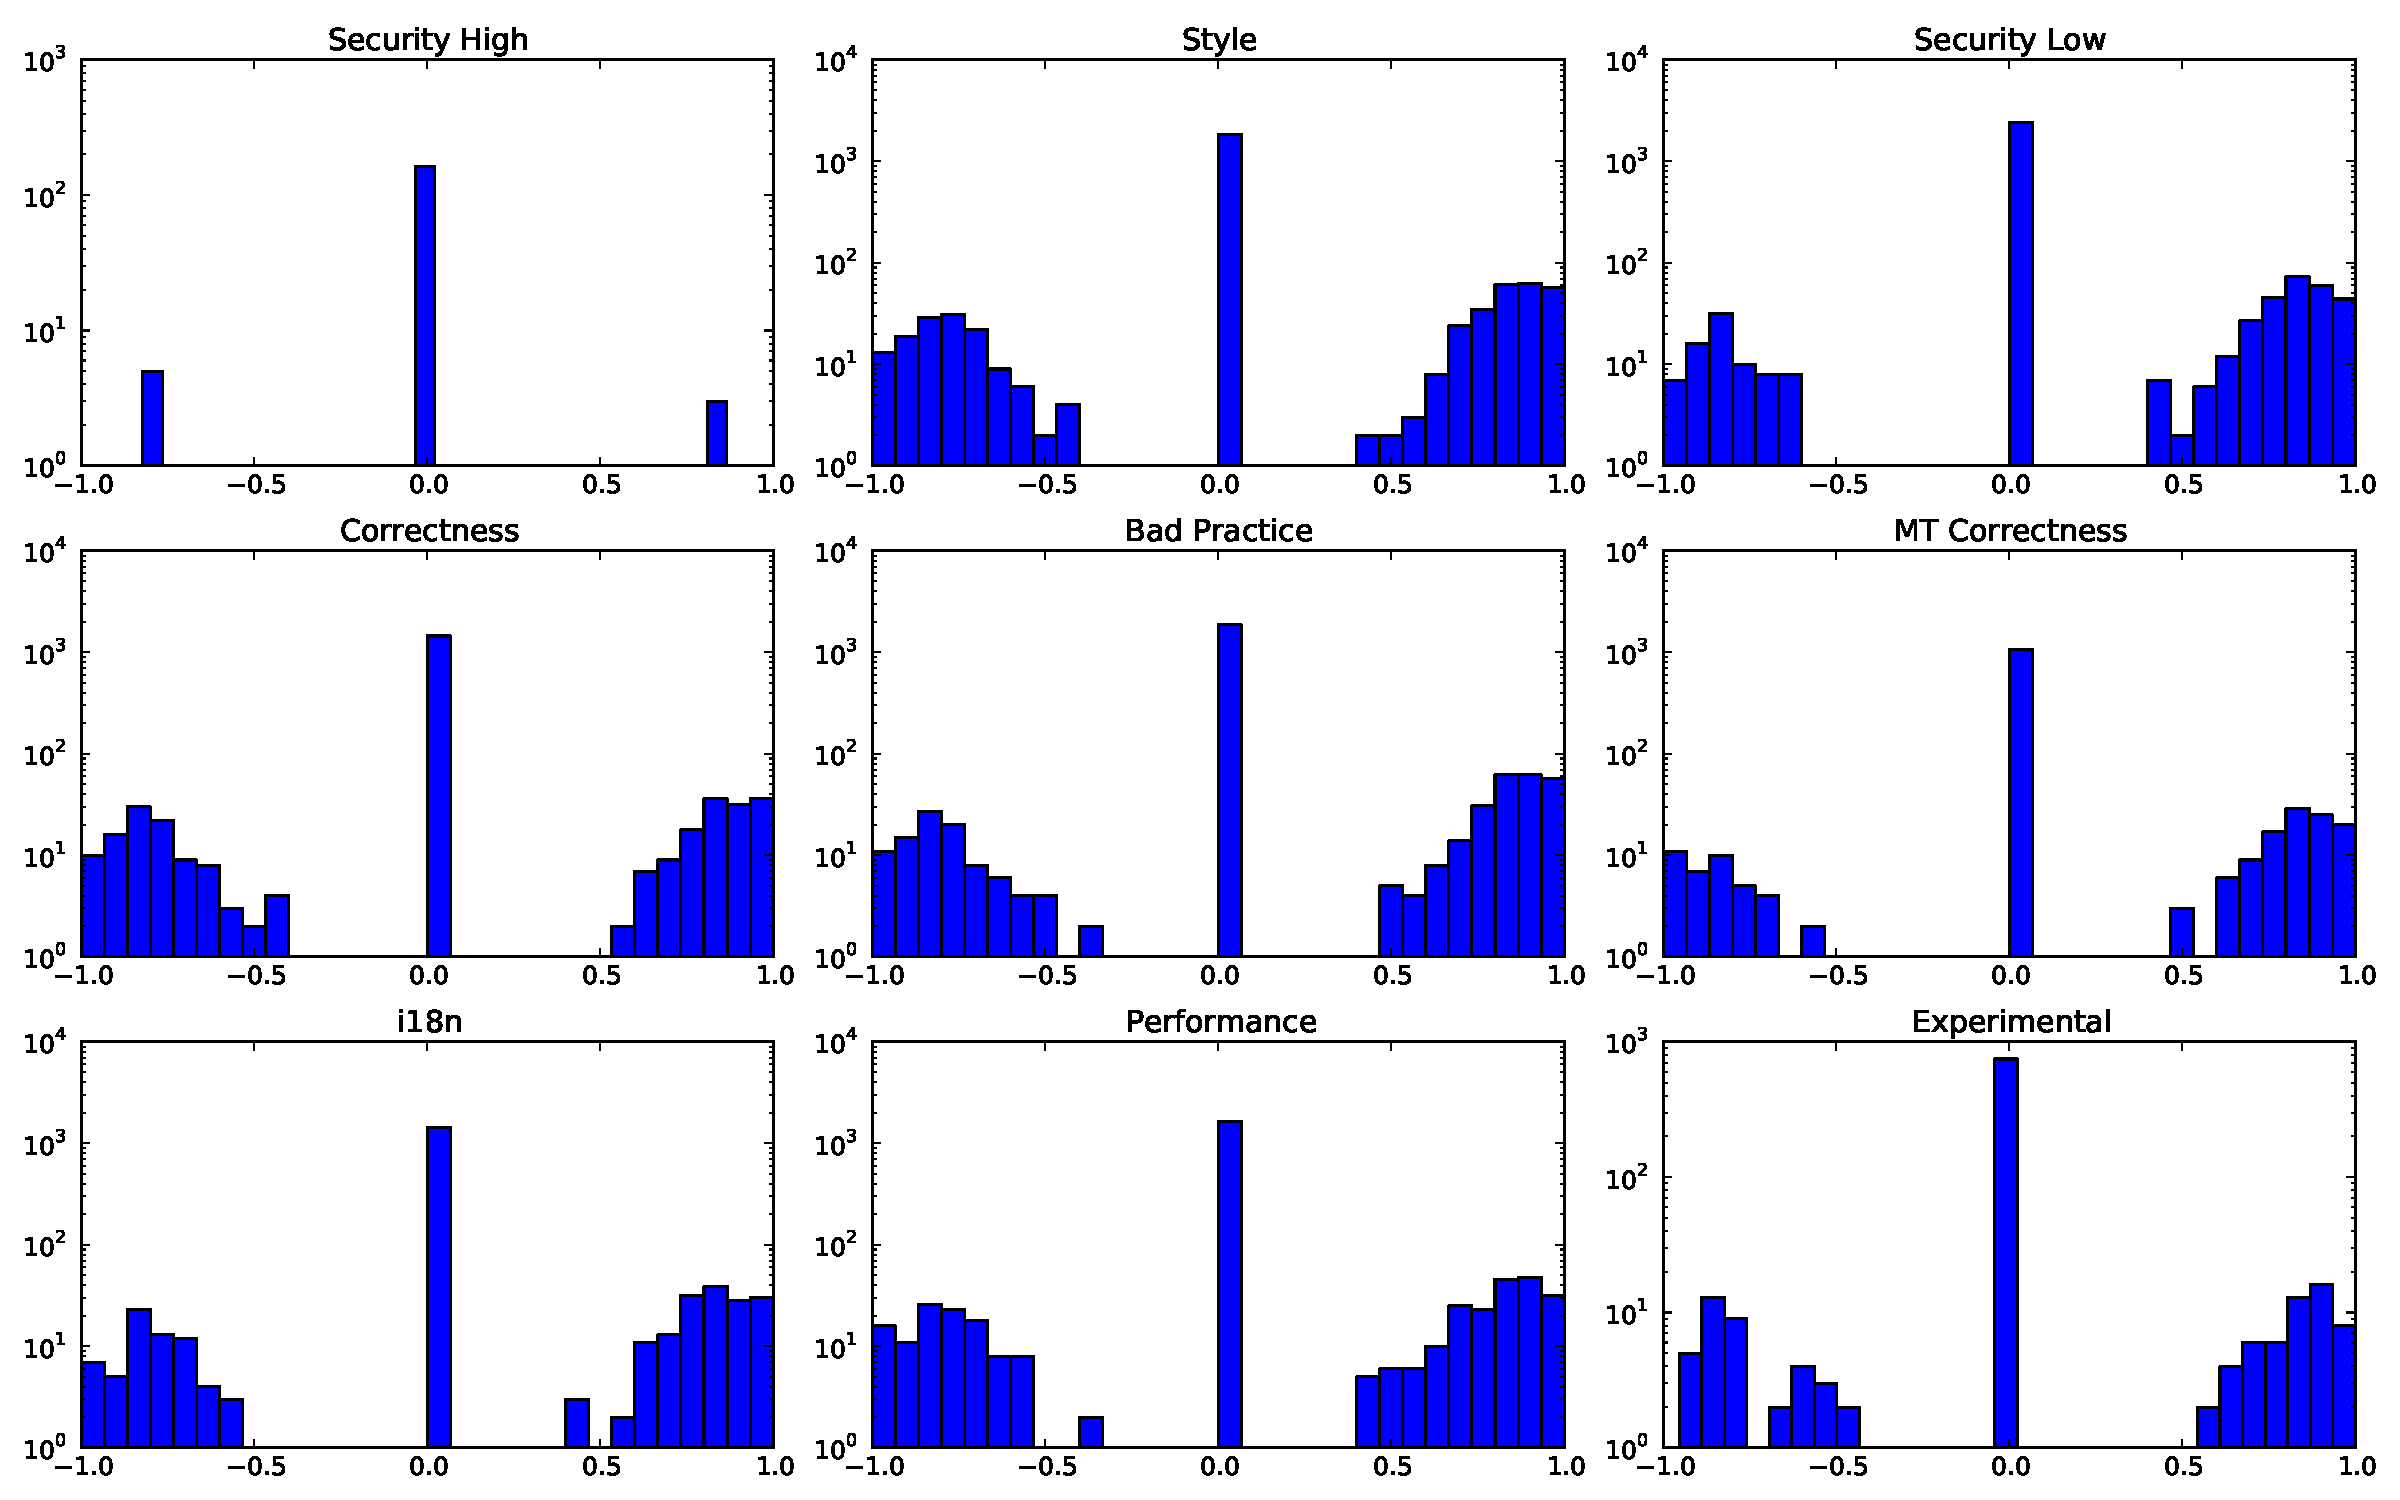
\includegraphics[scale=0.4]{bugsversionscorr}
  \caption{Histograms of correlations between bug counts and version
    ordinals per project. In brackets the total population size and
    the number of no correlation instances.}
  \label{fig:bugsversionscorr}
\end{figure*}

Another take on this theme is shown in Figure~\ref{fig:bugdiffs},
which presents an histogram of the changes of different bug counts in
project versions. In most cases, a bug count does not change between
versions; but when it does change, it may change upwards or downwards.
Note also the spectacular changes of introducing or removing thousands
of defects; this may be the result of doing and undoing a pervasive
code change that falls foul of some bug identification rule.

\begin{figure*}
  \centering
  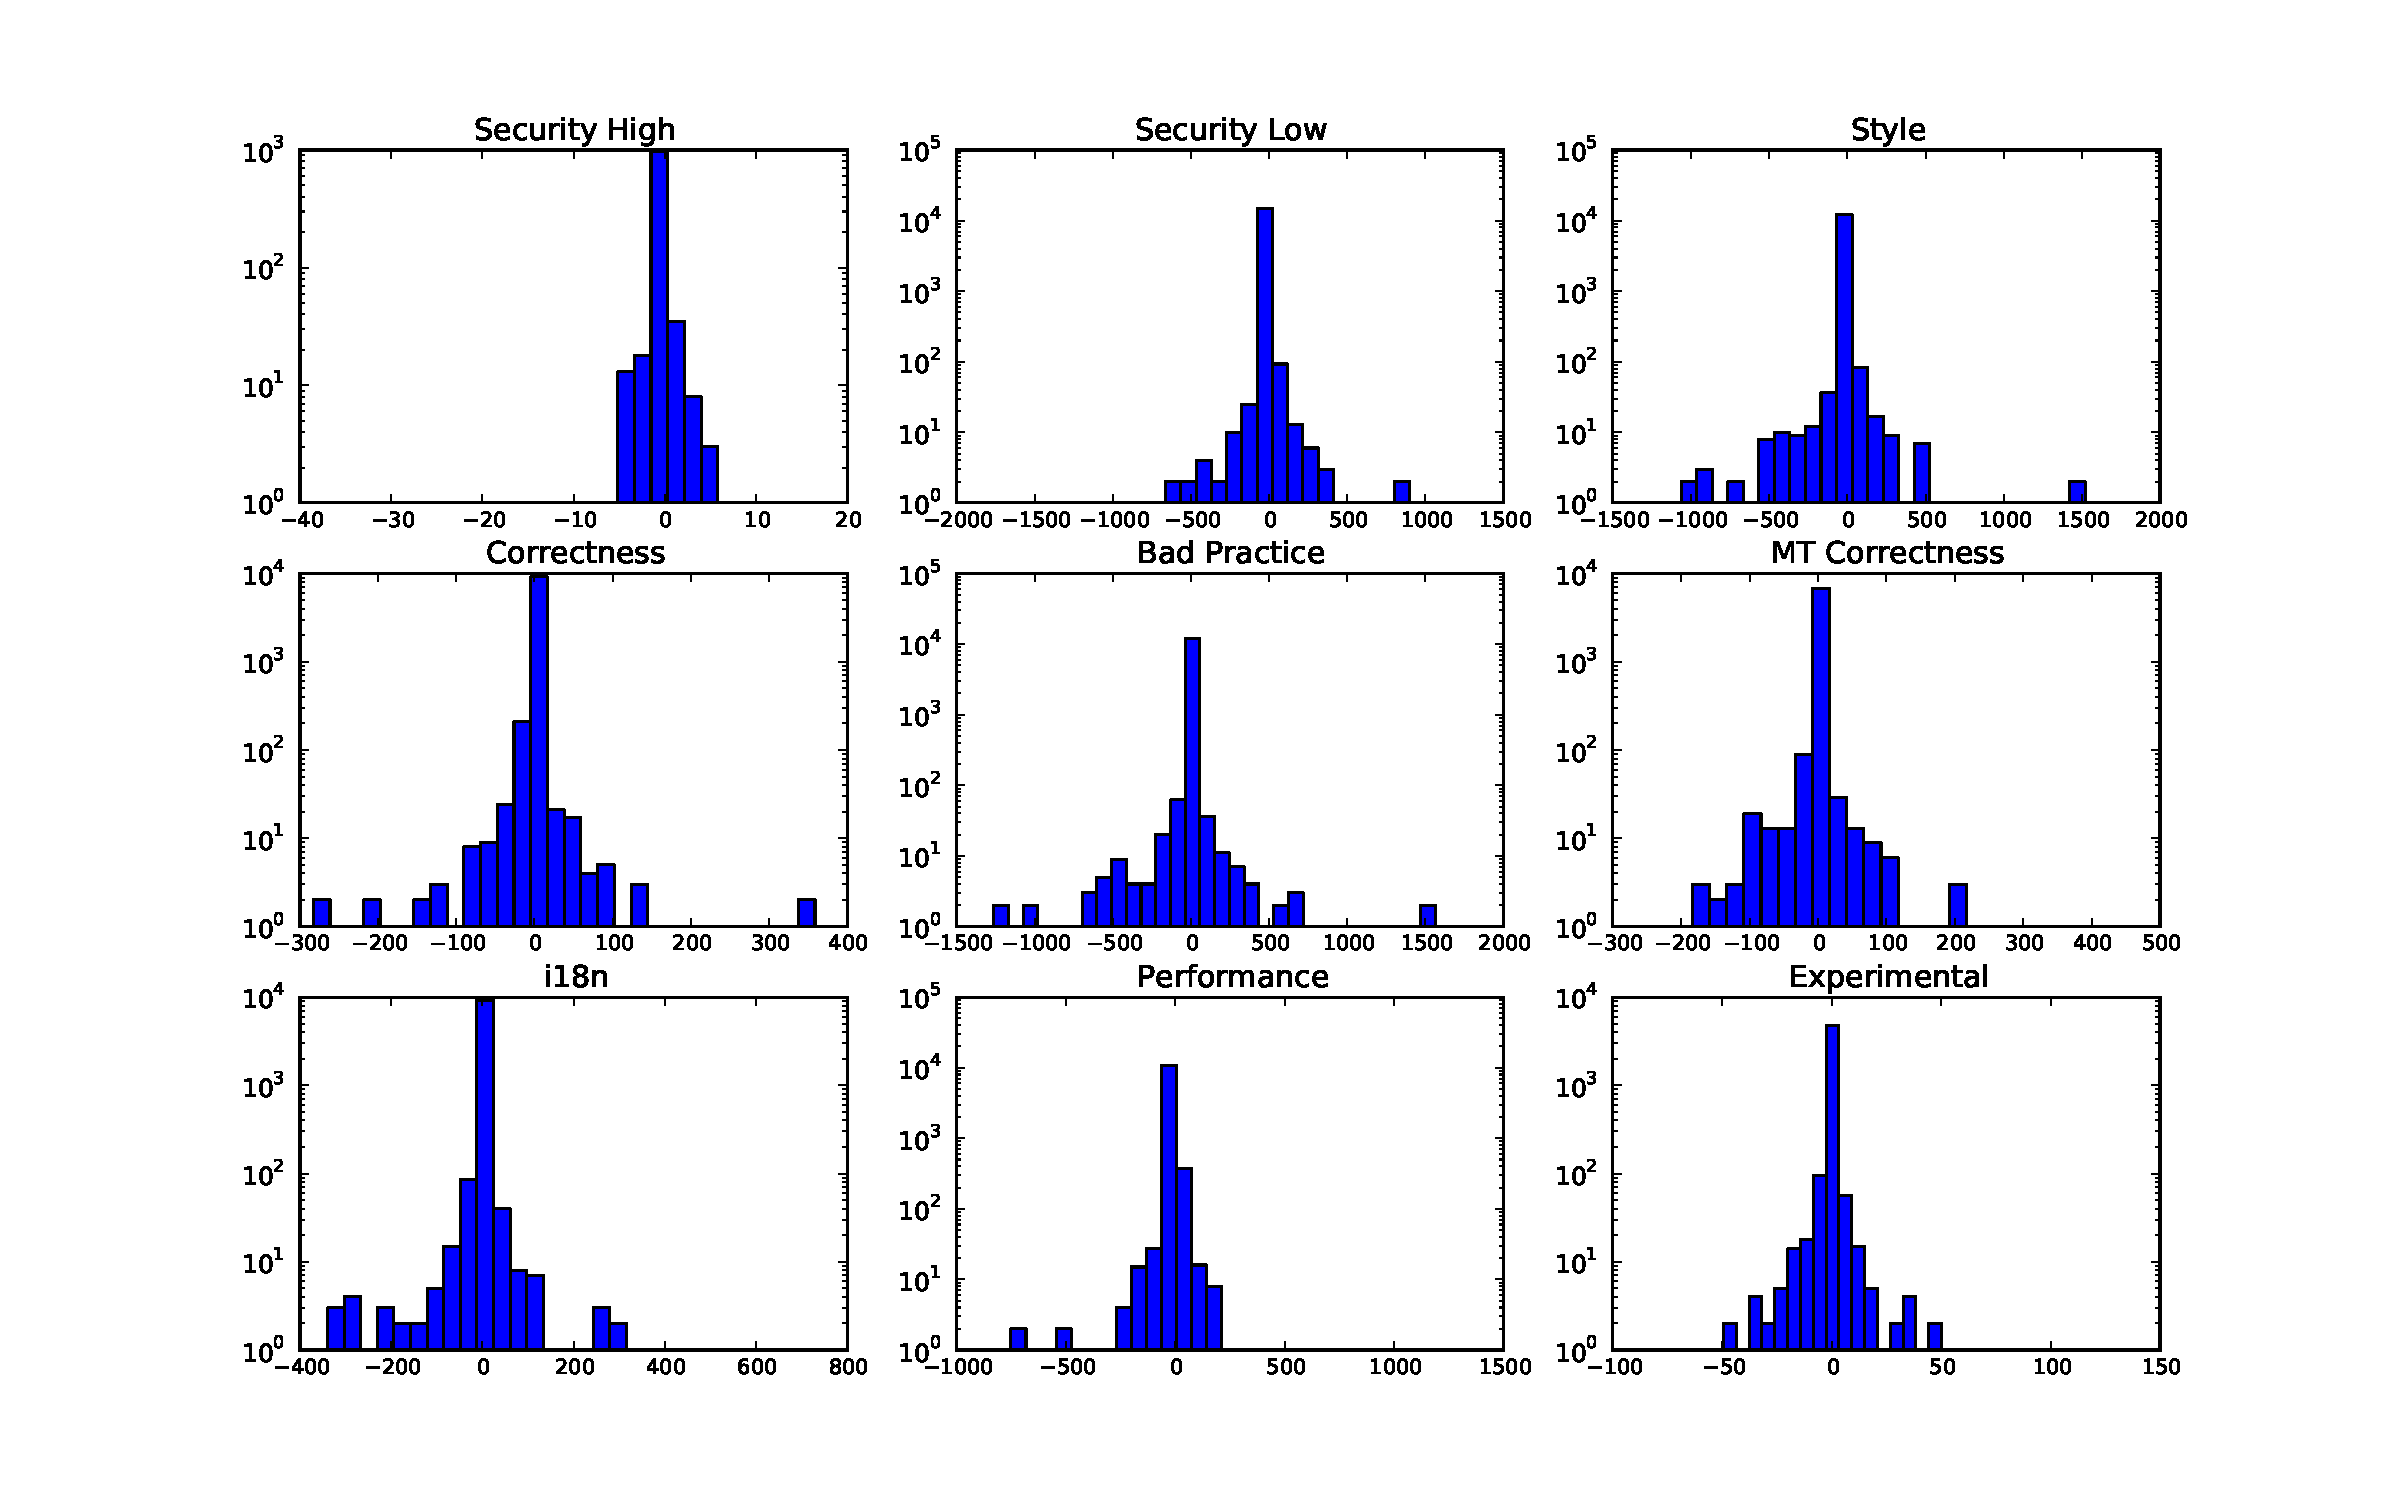
\includegraphics[scale=0.4]{bugdiffs}
  \caption{Histograms of the time, measure in versions, it takes for a
    bug to be closed. }
  \label{fig:bugdiffs}
\end{figure*}


\subsubsection{Persistence of Security Bugs}

To examine the relation between the persistence of different kinds of
bugs, and of security bugs in particular, we used as a persistence
indicator the number of versions a bug remains open in a project. We
grouped the persistence numbers by bug categories and then performed a
Mann-Whitney $U$ test among all bug category pairs. The results are
presented in Table~\ref{tbl:bug_persistence}. Cells in brackets show
pairs where no statistically significant difference was found.

In general, although the average number of versions bugs in different
bug categories remained opened was statistically different in many
cases, the difference is not spectacular. In all cases a bug persists
on average between two and three versions, with the difference being
in the decimal digits.

\begin{landscape}
  \begin{table}
    \setlength{\extrarowheight}{0.10cm}
    \caption{Bug Persistence Comparison}
    \label{tbl:bug_persistence}
    \resizebox{0.95\columnwidth}{!}{
    
\begin{tabular}{|l|>{\centering\arraybackslash}m{2.5cm}|>{\centering\arraybackslash}m{2.5cm}|>{\centering\arraybackslash}m{2.5cm}|>{\centering\arraybackslash}m{2.5cm}|>{\centering\arraybackslash}m{2.5cm}|>{\centering\arraybackslash}m{2.5cm}|>{\centering\arraybackslash}m{2.5cm}|>{\centering\arraybackslash}m{2.5cm}|}
\hline 
Security High & {\it ($0.04$, $p = 0.97$\newline 2.72, 2.36\newline 243, 35048)} & $2.22$, $p < 0.05$\newline 2.72, 2.12\newline 243, 49043 & {\it ($-0.51$, $p = 0.61$\newline 2.72, 2.50\newline 243, 12905)} & $2.77$, $p < 0.01$\newline 2.72, 2.11\newline 243, 49324 & {\it ($1.02$, $p = 0.31$\newline 2.72, 2.48\newline 243, 10227)} & {\it ($-1.19$, $p = 0.23$\newline 2.72, 2.74\newline 243, 10718)} & {\it ($-1.00$, $p = 0.32$\newline 2.72, 2.65\newline 243, 23598)} & {\it ($-0.33$, $p = 0.74$\newline 2.72, 2.85\newline 243, 2686)}\\
Security Low &  & $20.27$, $p \ll 0.05$\newline 2.36, 2.12\newline 35048, 49043 & $-3.59$, $p \ll 0.05$\newline 2.36, 2.50\newline 35048, 12905 & $25.17$, $p \ll 0.05$\newline 2.36, 2.11\newline 35048, 49324 & $5.59$, $p \ll 0.05$\newline 2.36, 2.48\newline 35048, 10227 & $-7.55$, $p \ll 0.05$\newline 2.36, 2.74\newline 35048, 10718 & $-8.19$, $p \ll 0.05$\newline 2.36, 2.65\newline 35048, 23598 & {\it ($-1.39$, $p = 0.17$\newline 2.36, 2.85\newline 35048, 2686)}\\
Style &  &  & $-17.96$, $p \ll 0.05$\newline 2.12, 2.50\newline 49043, 12905 & $5.66$, $p \ll 0.05$\newline 2.12, 2.11\newline 49043, 49324 & $-6.84$, $p \ll 0.05$\newline 2.12, 2.48\newline 49043, 10227 & $-20.61$, $p \ll 0.05$\newline 2.12, 2.74\newline 49043, 10718 & $-26.18$, $p \ll 0.05$\newline 2.12, 2.65\newline 49043, 23598 & $-8.30$, $p \ll 0.05$\newline 2.12, 2.85\newline 49043, 2686\\
Correctness &  &  &  & $21.38$, $p \ll 0.05$\newline 2.50, 2.11\newline 12905, 49324 & $7.44$, $p \ll 0.05$\newline 2.50, 2.48\newline 12905, 10227 & $-3.57$, $p \ll 0.05$\newline 2.50, 2.74\newline 12905, 10718 & $-2.91$, $p < 0.01$\newline 2.50, 2.65\newline 12905, 23598 & {\it ($0.40$, $p = 0.69$\newline 2.50, 2.85\newline 12905, 2686)}\\
Bad Practice &  &  &  &  & $-10.02$, $p \ll 0.05$\newline 2.11, 2.48\newline 49324, 10227 & $-23.63$, $p \ll 0.05$\newline 2.11, 2.74\newline 49324, 10718 & $-30.32$, $p \ll 0.05$\newline 2.11, 2.65\newline 49324, 23598 & $-9.98$, $p \ll 0.05$\newline 2.11, 2.85\newline 49324, 2686\\
MT Correctness &  &  &  &  &  & $-10.17$, $p \ll 0.05$\newline 2.48, 2.74\newline 10227, 10718 & $-10.83$, $p \ll 0.05$\newline 2.48, 2.65\newline 10227, 23598 & $-4.03$, $p \ll 0.05$\newline 2.48, 2.85\newline 10227, 2686\\
i18n &  &  &  &  &  &  & {\it ($1.29$, $p = 0.20$\newline 2.74, 2.65\newline 10718, 23598)} & $2.46$, $p < 0.05$\newline 2.74, 2.85\newline 10718, 2686\\
Performance &  &  &  &  &  &  &  & {\it ($1.92$, $p = 0.05$\newline 2.65, 2.85\newline 23598, 2686)}\\
\hline
\multicolumn{1}{l|}{}  &  &  &  &  &  &  &  &  \\
\cline{1-1}
\multicolumn{2}{l|}{Security Low}  &  &  &  &  &  &  &  \\
\cline{1-2}
\multicolumn{3}{l|}{Style}  &  &  &  &  &  &  \\
\cline{1-3}
\multicolumn{4}{l|}{Correctness}  &  &  &  &  &  \\
\cline{1-4}
\multicolumn{5}{l|}{Bad Practice}  &  &  &  &  \\
\cline{1-5}
\multicolumn{6}{l|}{MT Correctness}  &  &  &  \\
\cline{1-6}
\multicolumn{7}{l|}{i18n}  &  &  \\
\cline{1-7}
\multicolumn{8}{l|}{Performance}  &  \\
\cline{1-8}
\multicolumn{9}{l|}{Experimental}  \\
\cline{1-9}
\hline
\end{tabular}
}\\
    The matrix presents pairwise Mann-Whitney $U$ test results
    between the different bug categories. Each cell contains the test
    result (the value of $U$), the $p$-value, the average for each
    category and the sample size for each category. Cells in brackets show
    pairs where no statistically significant difference was found.
  \end{table}
\end{landscape}

\subsubsection{The Relation of Defects with the size of a {\sc jar}}

We explored the relation between defects with the size of a project version,
measured by the size of its {\sc jar} file by carrying out correlation tests
between the size and the defect counts for each project and its
version. The results, all statistically significant ($p \ll
0.05$) can be seen in Table~\ref{tbl:jarsizecorr}. The {\it Security
  High} category stands out by having a remarkably lower effect than
the other categories, even {\it Security Low} that nearly tops the
list. 

\begin{table}
    \centering
    \caption{Correlations between jar size and Defects Count}
    \label{tbl:jarsizecorr}
    
\begin{tabular}{lcc}
\hline \\
Category & Pearson Correlation & $p$-value \\ \hline 
Security High & 0.19 & $\ll 0.05$\\
Security Low & 0.64 & $\ll 0.05$\\
Style & 0.68 & $\ll 0.05$\\
Correctness & 0.56 & $\ll 0.05$\\
Bad Practice & 0.56 & $\ll 0.05$\\
MT Correctness & 0.55 & $\ll 0.05$\\
i18n & 0.43 & $\ll 0.05$\\
Performance & 0.57 & $\ll 0.05$\\
Experimental & 0.46 & $\ll 0.05$\\
\hline \\
\end{tabular}

\end{table}

\subsubsection{Security Bugs {\sc vs} Other Bug Categories}

To see whether bugs flock together we performed pairwise correlations
between all bug categories. We calculated the correlations between the
number of distinct bugs that appeared in a project throughout its
lifetime. The results can be seen in Table~\ref{tbl:corrmatrix} and
Figure~\ref{fig:corrplot}. We found significant, but not always
strong, correlations between all pairs. In general, the {\it Security
  High} category showed the weakest correlations with the other
categories. Our results show that in general bugs do flock together.
We do not find projects with only a certain kind of bug; bugs come
upon projects in swarms of different kinds. Bugs of the {\it Security
  High} category, though, are different: they are either not
associated with other bugs, or only weakly so. Perhaps it takes a
special kind of blunder to make it a security hazard.

\begin{table}
    \centering
    \caption{Correlation matrix}
    \label{tbl:corrmatrix}
    \begin{tabular}{ccccccccc}
\hline \\

1.00 & 0.27 & 0.19 & 0.12 & 0.17 & 0.43 & 0.13 & 0.23 & 0.24 \\
0.27 & 1.00 & 0.74 & 0.63 & 0.78 & 0.75 & 0.73 & 0.75 & 0.67 \\
0.19 & 0.74 & 1.00 & 0.68 & 0.77 & 0.68 & 0.70 & 0.72 & 0.61 \\
0.12 & 0.63 & 0.68 & 1.00 & 0.71 & 0.59 & 0.65 & 0.62 & 0.56 \\
0.17 & 0.78 & 0.77 & 0.71 & 1.00 & 0.73 & 0.84 & 0.84 & 0.77 \\
0.43 & 0.75 & 0.68 & 0.59 & 0.73 & 1.00 & 0.63 & 0.72 & 0.65 \\
0.13 & 0.73 & 0.70 & 0.65 & 0.84 & 0.63 & 1.00 & 0.80 & 0.70 \\
0.23 & 0.75 & 0.72 & 0.62 & 0.84 & 0.72 & 0.80 & 1.00 & 0.77 \\
0.24 & 0.67 & 0.61 & 0.56 & 0.77 & 0.65 & 0.70 & 0.77 & 1.00 \\

\hline \\
\end{tabular}


    \\
    \small The matrix presents pairwise correlations between the
        different bug categories.
\end{table}


\begin{figure*}
  \centering
  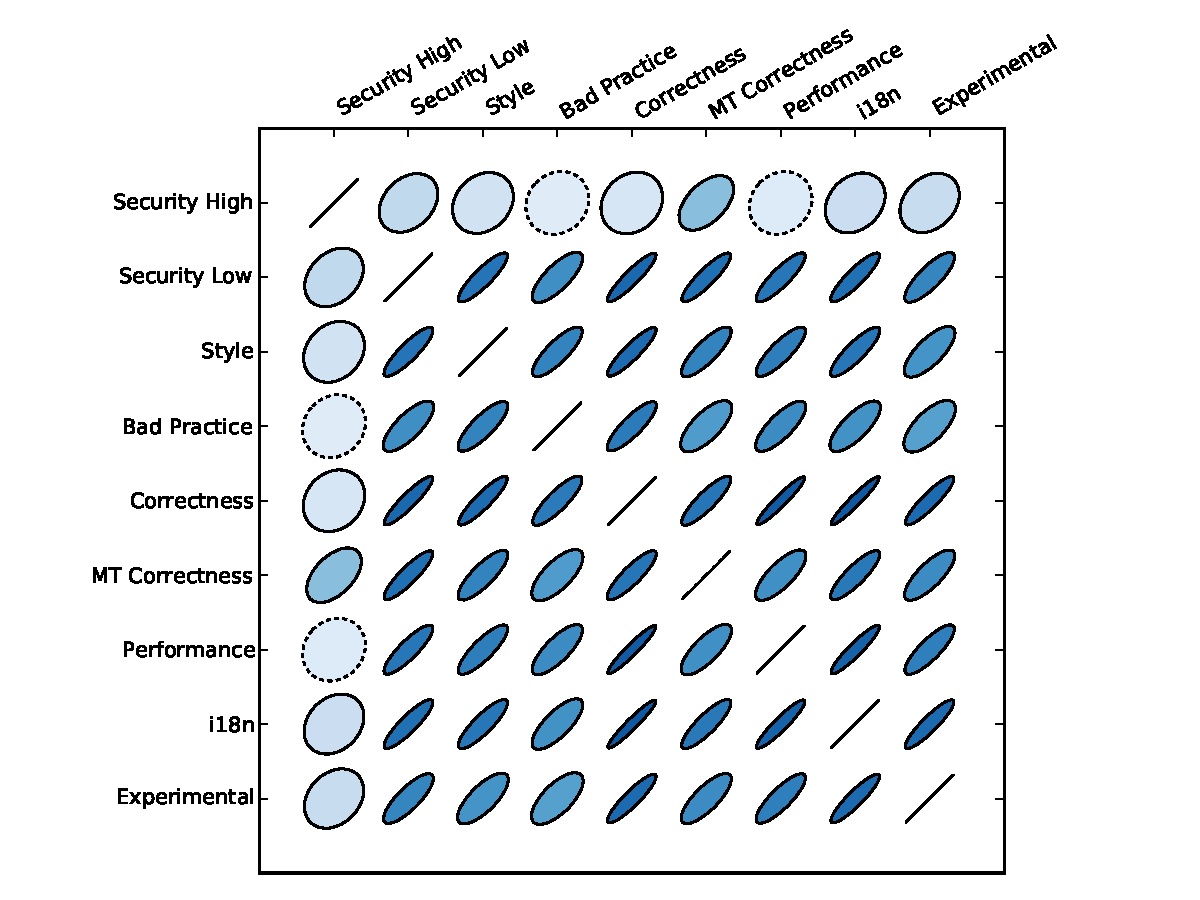
\includegraphics[scale=0.6]{corrplot.pdf}
  \caption{Correlation matrix plot for bug categories}
  \label{fig:corrplot}
\end{figure*}

\section{Discussion}
\label{sec:dis}
% also mention:
% - the fact that we don't have the same number of versions in every project.
% - tell about the graph and Linus.

By examining Maven as a whole we observed that security bugs and the
bugs coming from the {\it Bad Practice} category are the most popular types of
bugs in the ecosystem. This could be a strong indication that programmers write code
that implements the required functionality without considering its many
security aspects; an issue that has already been reported in
literature~\cite{SH09}. In addition, contrary to the Linus' Law, from the top fifty versions
(based on their PageRank), twenty five of them were the latest versions at the
time and at the same time contained security bugs.
This also highlights the {\it domino effect}~\cite{TH04}. No matter how well a programmer
secures a software component it won't matter if he or she is using vulnerable
code fragments from another library. Finally, 5,355 versions ($\approx 4,64\% $), contained at
least one severe security bug. Given the fact that other projects include these
versions as their dependencies, they are automatically rendered vulnerable if
they use the code fragments that include the defects. Finally, as
bug descriptions indicate,\footnote{\url{http://findbugs.sourceforge.net/bugDescriptions.html}}
if an application has bugs coming from the {\it Security High} category,
it might have more vulnerabilities that FindBugs doesn't report.



\section{Related Work}
\label{sec:rel}

There are numerous methods for mining software repositories in the context
of software evolution~\cite{KCM07}. In this section we focus on the ones
that highlight the relationship between software bugs and evolution and try to
extract useful conclusions. The key idea behind this concept is
similar to ours: the combination of information like bug descriptions,
documentation and others with the information retrieved from either the source
or object code of a project version.

{\it Refactoring identification} through software evolution is an approach used to
relate refactorings with software bugs. Wei{\ss}gerber et al. found that a high
ratio of refactorings is usually followed by an increasing ratio of bug
reports~\cite{WD06}. In addition, they indicated that software bugs are sometimes introduced
after an incomplete refactoring~\cite{GW05}.
Ratzinger et al.~\cite{RSG08} showed that the number of bugs decreases, when the number of
refactorings increases. Finally, Kim M. et al.~\cite{KCK11} indicated that {\sc api}-level
refactorings aid bug fixes.

Using {\it micro patterns} is a method proposed by Kim et al.~\cite{KPW06}
to detect bug-prone patterns among source code. Micro patterns describe programming
idioms like inheritance, data management, immutability and others. The approach involved
the examination of all revisions of three open-source projects to extract bug
introduction rates for each pattern. Gil et al.~\cite{GM05} analysed the
prevalence of micro patterns across five Sun {\sc jdk} versions to conclude that
pattern prevalence tends to be the same in software collections.

{\it Querying techniques} are used to answer a broad range of questions
regarding the evolution history of a project~\cite{HG05}. Bhattacharya et
al.~\cite{BN11}\cite{B11} proposed a framework that is based upon
recursively enumerable languages. The framework can correlate software
bugs with developers in various ways. For instance, return the list of
bugs fixed by a specific developer. Fischer et al.~\cite{FPG03} proposed
an approach for populating a release history database that combines code
information with bug tracking data. In this way, a developer can couple files
that contain common bugs, estimate code maturity with respect to the bugs
and others. The ``Ultimate Debian Database''~\cite{NZ10} is an {\sc sql}-based
framework that integrates information about the Debian project from various
sources to answer queries related to software bugs and source code.

D'Ambros et al. have used {\it bug history analysis} to detect
the critical components of a project~\cite{D08}. This is done by using an
evolutionary meta-model~\cite{DL08}. The same approach was
also used by Zimmermann et al.~\cite{ZNA08} to check the correlation
of bugs with software properties like code complexity, process quality and others
and predict future properties.

The evolution of software artifacts has also been analysed to {\it reduce the false
alarms} of the various static analysis tools. To achieve this, Spacco et
al.~\cite{SHP06} introduced {\it pairing} and {\it warning signatures}. In the
former, they tried to pair sets of bugs between versions in order to find
similar patterns. In the latter, they computed a signature for every bug. This
signature contained elements like the name of the class where the bug was found,
the method and others. Then they searched for similar signatures between
versions. In their research they also studied the evolution of 116 sequential
builds of the Sun Java Sevelopment Kit ({\sc jdk}). Their findings indicated that
high priority bugs are fixed over time. To improve the precision of bug
detection, Kim et al.~\cite{KE07b}\cite{KE07} proposed a history-based warning
prioritization algorithm by mining the history of bug-fixes of three
different projects. The algorithm was based on the following hypothesis: if a
bug that belongs to a specific category is eliminated by a code change, then
this warning category is important. Working towards the same direction, Heckman
et al.~\cite{HW09}\cite{HW08} have introduced benchmarks that use specific
correlation algorithms and classification techniques to evaluate alert
prioritization approaches.

Lu et al.~\cite{LAAL13} studied the {\it evolution of file-system code}.
Specifically, they analysed the changes of Linux file-system patches to extract
bug patterns and categorize bugs based on their impact. Their findings
indicated that the number of file-system bugs does not die down over time. By
categorizing bugs they also showed the frequency of specific bugs in specific
components.

Contrary to the above, our work focuses on the subset of security bugs.
Focusing on such bugs is not a new idea. Massacci et al.~\cite{MNN11} observed
the evolution of software defects by examining six major versions of Firefox.
To achieve this they created a database schema that contained information
coming from the ``Mozilla Firefox-related Security Advisories'' ({\sc mfsa})
list,\footnote{\url{http://www.mozilla.org/projects/security/known-vulnerabilities.html}}
Bugzilla entries and others. Their findings indicated that security bugs are
persistent over time. They also showed that there are many web users that use
old versions of Firefox, meaning that old attacks will continue to work.
Zaman et al.~\cite{ZAH11} focused again on Firefox to study the relation of
security bugs with performance bugs. This was also done by analysing the project's
Bugzilla. Their research showed that security bugs require more experienced developers
to be fixed. In addition, they suggested that security bug fixes are more complex than the
fixes of performance and other bugs.
Shahzad et al.~\cite{SSL12} analysed large sets of vulnerability data-sets to observe
various features of the vulnerabilities that they considered critical. Such features
were the functionality and the criticality of the defects. Their analysis
included the observation of vulnerability disclosures, the behavior of
hackers in releasing exploits for vulnerabilities, patching and others. In
their findings they highlighted the most exploited defects and showed that
the percentage of remotely exploitable vulnerabilities has gradually increased
over the years.

\section{Conclusions and Future Work}
\label{sec:con}

Our work could (?) aid bug-prediction models in the same way as~\cite{BN11}.

\section*{Acknowledgements}

This research has been co-financed by the European Union (European Social Fund
--– {\sc esf}) and Greek national funds through the Operational Program
``Education and Lifelong Learning'' of the National Strategic Reference Framework –
Research Funding Program: Heracleitus II. Investing in knowledge society
through the {\sc esf}.

The project has been also co-financed by the European Regional Development Fund ({\sc erdf})
and national funds and is a part of the Operational Programme ``Competitiveness \&
Entrepreneurship" ({\sc opce} II), Measure ``{\sc cooperation}" (Action I).

\bibliographystyle{splncs}
\bibliography{evol} 

\end{document}


